

% \title{Inkscape package on Overleaf }
\chapter{The PricingPy Python Library}
\section{Implementation in vectorial form}
In the previous chapter we showed the full model and expressed in such a simple final equation that it can be stated directly in vectorial form in Python or any programmatic language with support for matrix algebra.\\

For illustration purposes, consider the computation given in equation (\ref{eq:bbar1}). To implement that we will define the following vectors:
\begin{align}
T = \begin{bmatrix} 
    T_{1} & \dots &  T_{m} \\
    \end{bmatrix}    
\end{align}
\begin{align}
r = \begin{bmatrix} 
    r_{1} & \dots &  r_{m} \\
    \end{bmatrix}    
\end{align}
\begin{align}
disb = \begin{bmatrix} 
    d_{1} & \dots &  d_{m} \\
    \end{bmatrix}    
\end{align}
\begin{align}
T^{mat} = \begin{bmatrix} 
     1  \\
     2  \\
    \vdots  \\
    T^{max} 
    \end{bmatrix}       
\end{align}
With the definitions above, $\bar{B}$ can be diretly computed using equation (\ref{eq:bbar1}) and array broadcasting operators in numpy:

\begin{align}
    \bar{B} = disb*\frac{(1+r)^{T^{max}}-(1+r)^{T^{mat}-1}}{(1+r)^{T^{max}}-1}
\end{align}
With this approach $\bar{B}$ results of order $T^{max}\times m$ as expected.
\begin{align}
\bar{B} = \begin{bmatrix} 
    b_{1,1} & \dots &  b_{1,m} \\
    \vdots & \ddots & \\
    b_{T^{max},1} &        & b_{T^{max},m} 
    \end{bmatrix}    
\end{align}
\section{Class Diagram}
The pattern design is following the pattern detailed in Buitinck et al (2013)  \cite{scikitlearn-2013}. An extraordinary reference is G\'eron (2019) \cite{geron2019}
\begin{figure}[H]
  \centering
      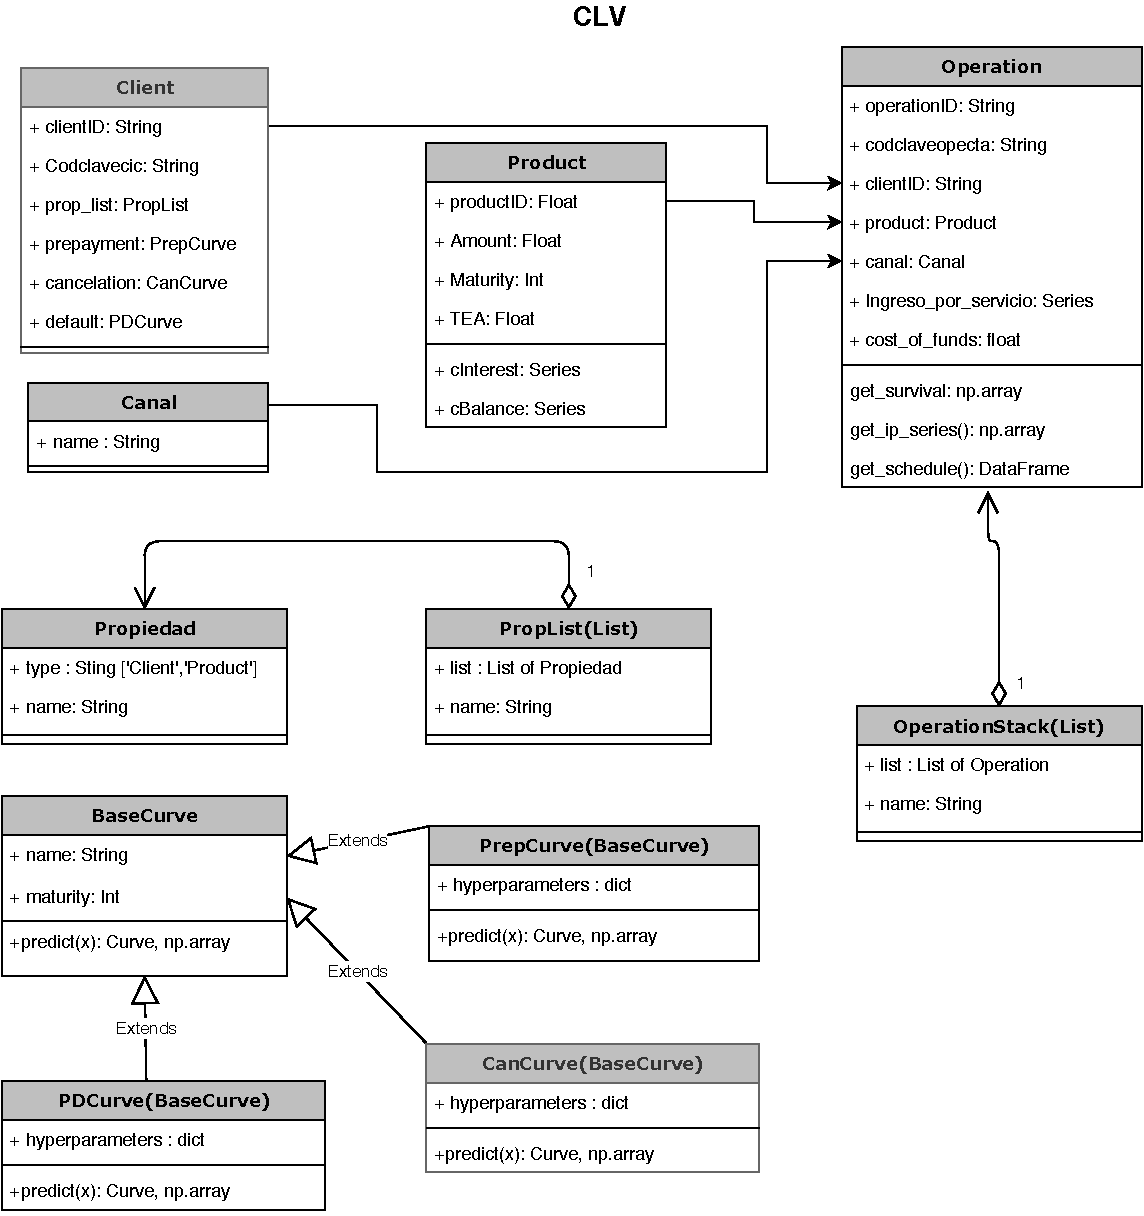
\includegraphics[width=1\textwidth]{diagrCLV.pdf} 
 \caption{CLV Class Diagram}
 \label{fig:TestCD}
\end{figure}

\begin{figure}[H]
  \centering
      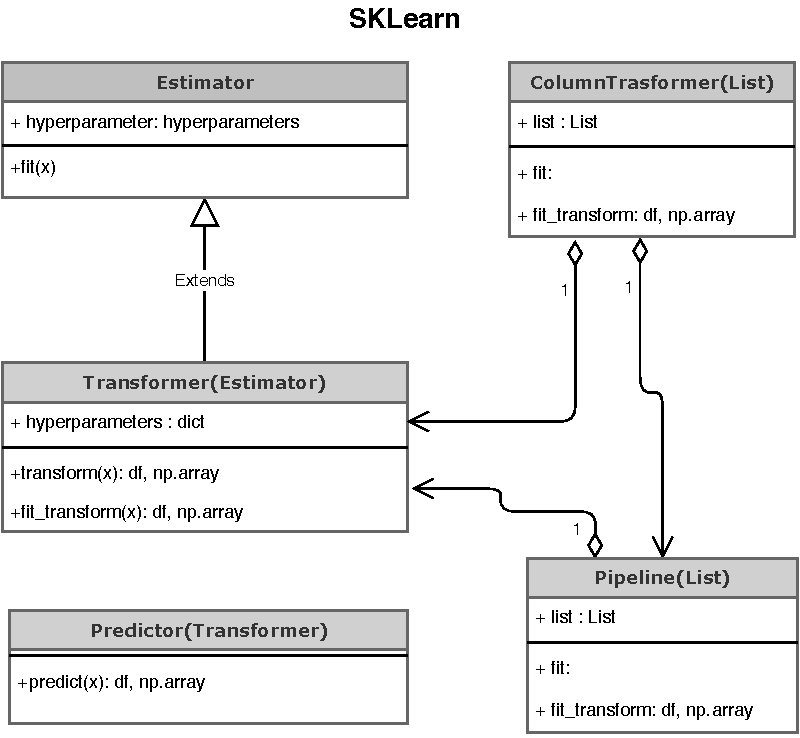
\includegraphics[width=.6\textwidth]{diagrSklearn.pdf} 
 \caption{SKLearn Class Diagram}
 \label{fig:TestSCD}
\end{figure}

